%%%  Ukázkový text a dokumentace stylu pro text závěrečné (bakalářské a
%%%  diplomové) práce na KI PřF UP v Olomouci
%%%  Copyright (C) 2012 Martin Rotter, <rotter.martinos@gmail.com>
%%%  Copyright (C) 2014 Jan Outrata, <jan.outrata@upol.cz>


%%  Pro získání PDF souboru dokumentu je třeba tento zdrojový text v
%%  LaTeXu přeložit (dvakrát) programem pdfLaTeX.

%%  V případě použití programu BibLaTeX pro tvorbu seznamu literatury
%%  je poté ještě třeba spustit program Biber s parametrem jméno
%%  souboru zdrojového textu bez přípony a následně opět (dvakrát)
%%  přeložit zdrojový text programem pdfLaTeX.

%%  Postup získání Postscriptového souboru je popsán v dokumentaci.


%%  Třída dokumentu implementující styl pro závěrečnou práci. Vybrané
%%  nepovinné parametry (ostatní v dokumentaci):

%%  'master' pro sazbu diplomové práce, jinak se sází bakalářská práce

%%  'field=kód' pro Váš studijní obor, kódy pro diplomovou práci 'uvt'
%%  pro Učitelství výpočetní techniky pro střední školy a 'binf' pro
%%  Bioinformatiku, jinak je výchozí Informatika, a pro bakalářskou
%%  práci 'ainfk' pro Aplikovanou informatiku v kombinované formě,
%%  'inf' pro Informatiku, 'infv' pro Informatiku pro vzdělávání a
%%  'binf' pro Bioinfomatiku, jinak je výchozí Aplikovaná informatika
%%  v prezenční formě

%%  'printversion' pro sazbu verze pro tisk (nebarevné logo a odkazy,
%%  odkazy s uvedením adresy za odkazem, ne odkazy do rejstříku),
%%  jinak verze pro prohlížeč

%%  'biblatex' pro zapnutí podpory pro sazbu bibliografie pomocí
%%  BibLaTeXu, jinak je výchozí sazba v prostředí thebibliography

%%  'language=jazyk' pro jazyk práce, jazyky english pro anglický,
%%  slovak pro slovenský, jinak je výchozí czech pro český

%%  'font=sans' pro bezpatkový font (Iwona Light), jinak výchozí
%%  patkový (Latin Modern)

\documentclass[
%  master,
%  field=inf,
%  printversion,
  biblatex,
%  language=english,
%  font=sans,
  glossaries,
  index
]{kidiplom}

\usepackage{algorithm,algorithmicx,algpseudocode}

%% Informace pro úvodní strany. V jazyku práce (pokud není v komentáři
%% uvedeno česky) a anglicky. Uveďte všechny, u kterých není v
%% komentáři uvedeno, že jsou volitelné. Při neuvedení se použijí
%% výchozí texty. Text pro jiný než nastavený jazyk práce (nepovinným
%% parametrem language makra \documentclass, výchozí český) se zadává
%% použitím makra s uvedením jazyka jako nepovinného parametru.

%% Název práce, česky a anglicky. Měl by se vysázet na jeden řádek.
\title{Editor Petriho Sítí}
\title[english]{Petri Nets Editor}

%% Volitelný podnázev práce, česky a anglicky. Měl by se vysázet na
%% jeden řádek. Výchozí je prázdný.
\iffalse
\subtitle{Ukázkový text a dokumentace stylu v \LaTeX{}u}
\subtitle[english]{Sample text and documentation of the \LaTeX{} style}
\fi

%% Jméno autora práce. Makro nemá nepovinný parametr pro uvedení
%% jazyka.
\author{Roman Wehmhöner}

%% Jméno vedoucího práce (včetně titulů). Makro nemá nepovinný
%% parametr pro uvedení jazyka.
\supervisor{Mgr. Petr Osička, Ph.D.}

%% Volitelný rok odevzdání práce. Výchozí je aktuální (kalendářní)
%% rok. Makro nemá nepovinný parametr pro uvedení jazyka.
%\yearofsubmit{\the\year}

%% Anotace práce, včetně anglické (obvykle překlad z jazyka
%% práce). Jeden odstavec!
\annotation{Cílem bakalářské práce bylo vytvořit editor 
  petriho sítí umožňující jednoduché a pohodlné ovládání. 
  Editor také obsahuje základní nástroje pro analýzu petriho 
  sítí. }

\annotation[english]{}

%% Klíčová slova práce, včetně anglických. Oddělená (obvykle) středníkem.
\keywords{styl textu; závěrečná práce; dokumentace; ukázkový text}
\keywords[english]{text style; thesis; documentation; sample text}

%% Volitelná specifikace příloh textu práce, i anglicky. Výchozí je '1
%% CD/DVD'.
%\supplements{jedno kulaté placaté CD/DVD s malou kulatou dírou uprostřed}
%\supplements[english]{one round flat CD/DVD with a small round hole in the middle}

%% Volitelné poděkování. Stručné! Výchozí je prázdné. Makro nemá
%% nepovinný parametr pro uvedení jazyka.
\thanks{Děkuji, děkuji, děkuji.}

%% Cesta k souboru s bibliografií pro její sazbu pomocí BibLaTeXu
%% (zvolenou nepovinným parametrem biblatex makra
%% \documentclass). Použijte pouze při této sazbě, ne při (výchozí)
%% sazbě v prostředí thebibliography.
\bibliography{bibliografie.bib}

%% Další dodatečné styly (balíky) potřebné pro sazbu vlastního textu
%% práce.
\usepackage{lipsum}


\usepackage{enumitem}
\newlist{steps}{enumerate}{1}
\setlist[steps, 1]{label = Krok \arabic*:}

\usepackage{graphicx}
\graphicspath{ {./images/} }

\usepackage{subcaption}
\usepackage[czech]{babel}

\begin{document}

%% Sazba úvodních stran -- titulní, s bibliografickými údaji, s
%% anotací a klíčovými slovy, s poděkováním a prohlášením, s obsahem a
%% se seznamy obrázků, tabulek, vět a zdrojových kódů (pokud jejich
%% sazba není vypnutá).
\maketitle

%% Vlastní text závěrečné práce. Pro povinné závěry, před přílohami,
%% použijte prostředí kiconclusions. Povinná je i příloha s obsahem
%% přiloženého CD/DVD.

%% -------------------------------------------------------------------

\newcommand{\BibLaTeX}{\textsc{Bib}\LaTeX}



















\newcommand{\todo}[1]{\textcolor{red}{TODO: #1}\PackageWarning{TODO:}{#1!}}
\todo{Smazat todo: command}

\section{Petriho sítě}
Táto kapitola byla inspirovaná a čerpala informace z knihy Understanding petri nets\cite{reisig2013understanding}

\subsection{Základní popis}

Petriho síťe jsou matematickým nástrojem
pro modelování a simulaci paralelních procesů a jejich sychronizaci.
Jsou tvořené místy, přechody a hranami které jsou vždy propojením jednoho místa s jedním přechodem.

\begin{definition}[Petriho síť]
  $$ N = \langle P,T,A,M_{0}\rangle $$
  \begin{itemize}
    \item $N$ je Petriho sítí
    \item $P$ je konečná množina míst
    \item $T$ je konečná množina přechodů
    \item $A$ je konečná množina hran
        $ A \subseteq ((P \times T) \cup (T \times P)) \times \mathbb{N}_0 $ \\
        kde číslo symbolizuje násobek kolik značek hrana \uv{přesune}
        \item $M_{0} : P \rightarrow \mathbb{N}_0$ je počáteční ohodnocení sítě (zkráceně ohodnocení) míst
        kde pro každé místo $p \in P$ existuje počet jeho značek $m \in M_{0}$
  \end{itemize}
\end{definition}

Pro odkazovaní na jednotlivé členy prvků z množiny hran budeme používat
notaci $P(a)$ pro odkázání na místo v hraně $a \in A$,
$T(a)$ pro odkázání na přechod a $AM(a)$ pro odkaz na násobek.

Každý přechod $t$ může mít 'přiřazený' libovolný počet
hran, kde každá hrana $a$ je propojením s některým z míst $p \in P$.\\
Hrany přechodu $t$ můžeme rozlišit na hrany směrující do přechodu
$$^\to t = \{a \in A | a \in (P \times T \times \mathbb{N}_0) \land t = T(a)\}$$
a hrany směřující z přechodu (do místa)
$$ t ^\to  = \{a \in A | a \in (T \times P \times \mathbb{N}_0) \land t = T(a)\}$$
dohromady pak všechny hrany přechodu $t$ jsou spojením těchto dvou množin
$$ArcesOfTransition(t,A) = (^\to t \cup t ^\to) \subset A$$

Aktuální stav petriho sítě neboli ohodnocení M je funkce přiřazující každému
místu $p \in P$ petriho sítě počet značek
$$(\forall p \in P) M(p) \in \mathbb{N}_0$$
počáteční ohodnocení petriho sítě se značí $M_{0}$.

Pro dané ohodnocení $M$ je přechod $t \in T$ označený jako povolený
pokud všechny hrany směřující do přechodu $\,^\to t$ splňují svou podmínku tzn.
hrana splňuje svoji podmínku pokud místo ze kterého vychází má vyšší nebo stejné ohodnocení
(v daném $M$) než je násobek hrany $AM$
$$IsEnabled(P,t,A,M) = (\forall a \in \,^\to t)M(P(a)) \geq AM(a)$$
Pak si můžeme ještě definovat množinu všech povolených přechodů pro zadané ohodnocení
$$
  EnabledTransitions(P,T,A,M) =
  \{ t \in T | IsEnabled(P,t,A,M) \}
$$

Pokud je přechod $t$ v ohodnocení $M$ Petriho sítě \textbf{povolen}, znamená to že může dojít
k aktivování tohoto přechodu čímž dojde ke změně aktuálního ohodnocení z $M$ do ohodnocení $M'$
tak, že pro každé místo $p \in P$ a každou hranu $A_{pt} \subset ArcesOfTransition(t,A)$ spojující $p$ s $t$
že nové ohonocení v místě $M'(p)$ je sumou násobků hran $\sum_{a \in A_{pt}} AM(a)$ a původního hodnocení $M(p)$
$$
  FireTransition(P,t,A,M) = function\:M'
$$
Výsledné ohodnocení $M'$ je pak pro každé místo $p$ definováno
$$
  M'(p) = M(p) + \sum_{a \in \{a_{tp} \in ArcesOfTransition(t,A) \,|\, P(a_{tp}) = p \}} AM(a)
$$
Tuto změnu můžeme značit $M \to ^t M'$

Ohodnocení $M'$ je označené jako \textbf{dosažitelné}\index{dosažitelné ohodnocení} z ohodnocení $M$ 
pokud existuje sekvence přechodů taková, že jejich postupným aktivováním
z ohodnocení $M$ vznikne ohodnocení $M'$.
Ohdonocení $M'$ je dostupné z ohodnocení $M$ pak značíme $M \to ^* M'$.


\subsection{Vizuální zobrazení sítě}

Pro Petriho síť existuje nejenom matematické zobrazení ale i
v praxi více využívané grafické zobrazení. 
V grafickém zobrazení kolečka symbolizují místa petriho sítě
a číslo v kolečku udává počet značek. 
Přechody jsou symbolizované 
čtverci. V editoru je čtverec zelený pokud je přechod povolený.
Pokud má v sobě čtverec symbol $\epsilon$, znamená to že je 
přechod určený pro komunikaci sítě s okolním prostředím.
Na editor nemá žádný vliv jestli je přechod označený jako $\epsilon$
a tak tedy toto označení je jen pro jednoduší orientaci v síti.
Kolečka i čtverce mají pak nad sebou značení 
konkrétního místa/přechodu které symbolizují. 
Nakonec samotné hrany jsou symbolizované šipkamy které jsou 
popsané násobkem kolik hrana \uv{přesune} značek.
Popis hran je symbolizován dvěmi čísly oddělenými kolečkem.
Číslo před kolečkem značí hodnotu hrany směrující z přechodu 
do místa, číslo za kolečkem značí hodnotu hrany směrující z 
místa do přechodu.

Na obrázku \ref{fig:jednoduchá síť zobrazení} můžeme vidět grafické 
vyobrazení jednoduché sítě s dvěmi místy, třemi přechody a čtyřmi hranami.
\begin{figure}[h]
  \centering
  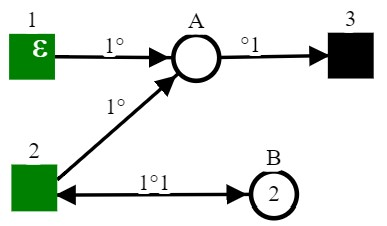
\includegraphics{simple_net}
  \caption[síť]{Příklad zobrazení jednoduché sítě}\label{fig:jednoduchá síť zobrazení}
\end{figure}
Již na první pohled si můžeme všimnou že pro jednoduší rozlišení 
míst a přechodů jsou přechody značené čísli a místa písmeny.
Tuto síť vyobrazenou na obrázku \ref{fig:jednoduchá síť zobrazení} 
bychom mohli matematickým zápisem zapsat jako síť 
$ N = \langle P,T,A,M_{0}\rangle $
kde \\
$P = \{a,b\}$ \\
$T = \{1,2,3\}$ \\
$A = \{
  \langle 1,a,1 \rangle,
  \langle 2,a,1 \rangle,
  \langle 2,b,1 \rangle,
  \langle b,2,2 \rangle,
  \langle a,3,1 \rangle
\}$ \\
$M_{0}(a) = 0; M_{0}(b) = 2$

V matematickém zápise sítě budeme místa značit malými písmeny (oproti editoru)
abychom předešli případným nedorozuměním.

\subsection{Zkrácený zápis ohodnocení sítě}

Abychom předešli zdlouhavému psaní kaźdého případu ohodnocovací funkce
(např. $M(a) = 0; M(c) = 2; \dotsb$), zavedeme si kratší zápis.
Nejdříve seřadíme všechny místa podle jejich značení jako by šlo 
o číselnou soustavu (s písmeny místo čísel) 
neboli $a, b, c, \dotsb, z, aa, ab, ac, \dotsb$.
Pak si z těchto míst uděláme uspořádanou n-tici jejich ohodnocení $\langle M(a), M(b), M(c), \dotsb \rangle$.
Tuto n-tici pak budeme používat jako kratší zápis ohodnocovací funkce:
$$
 M = \langle M(a), M(b), M(c), \dotsb \rangle
$$
Například pro $M'(a) = 3; M'(b) = 0; M'(c) = 5$ by krátký zápis vypadal
\\ $M' = \langle 3,0,5 \rangle$

\subsection{Využití Petriho sítí}

Petriho sítě se používají k analýze a modelování paralelních
a distribuovaných systému, databázových systémů atd. a to ať už
pro analýzu při vývoji softwaru a nebo pro popis vnitřńí struktury
již hotového proprietárního softwaru umožnující lepší porozumění uživateli.

\subsection{Graf dosažitelnosti}

Graf dosažitelnosti je jeden z nejzákladnějších nástrojů pro analýzu Petriho sítí.
Obsahuje vždy počáteční ohodnocení a všechny ohodnocení které jsou dostupné z počátečního ohodnocení, 
takovéto ohodnocení budeme nazývat \textbf{dosažitelné ohodnocení}\index{dosažitelné ohodnocení}. 
Vrcholy grafu jsou jednotlivá ohodnocení
a hrany grafu jsou značené přechody které jsou aktivované aby z počátečního ohodnocení vzniklo cílové.

\begin{definition}[Graf dosažitelnosti]
  $$RG = \{M, \langle M, T', M' \rangle\}$$
  \begin{itemize}
    \item $RG$ je Graf dosažitelnosti
    \item $M$ je Vrchol grafu který je zároveň konkrétní ohodnocení petriho sítě
    \item $\langle M, T', M' \rangle$ je Hrana grafu která je změnou z hodnocení $M$ libovolným přechodem $t \in T'$ ze kterého vzniká $M'$
  \end{itemize}
\end{definition}

\subsubsection{Vlastnosti odvoditelné z Grafu dosažitelnosti}
Z grafu dosažitelnosti Petriho sítě jsou odvoditelné tyto vlastnosti:

\begin{definition}
  
  Petriho síť je \textbf{ohraničená}\index{síť ohraničenost} pokud 
  je její graf dosažitelnosti konečný. Pokud existuje takové přirozené číslo $n$
  pro které v žádném dosažitelném ohodnocení nepřesahuje žádné místo svým ohodnocením 
  číslo $n$. Pokud zvolíme $n$ aby splňovalo tuto podmínku a zároveň bylo 
  nejmenší možné, pak můžeme nazývat síť že je \textbf{ohraničená $n$}.
  
\end{definition}
\begin{definition}\label{def:skončí}
  
  Petriho síť \textbf{skončí}\index{síť skončí} za předpokladu
  že graf je konečný a zároveň neobsahuje žádné cykly.
  Neboli Petriho sít vždy po nějakém počtu kroků dojde do stavu kdy žádný přechod není povolený.
  
\end{definition}
\begin{definition}
  
  Petriho síť je \textbf{vratná}\index{síť vratná}
  pokud je její graf silně souvislý. Z každého dosažitelného 
  ohdonocení je dosažitelné počáteční ohodnocení.

\end{definition}
\begin{definition}
  
  Petriho síť je \textbf{bez mrtvého bodu}\index{síť bez mrtvého bodu}
  pokud z každého vrcholu grafu dosažitelnosti vede alespoň jedna hrana.
  Petriho sít má v každém ohodnocení povolený alespoň jeden přechod.

\end{definition}
\begin{definition}
  
  Petriho síť je \textbf{slabě živá}\index{síť slabě živá} pokud pro
  každý přechod existuje v grafu hrana označená tímto přechodem.
  Pro každý přechod Petriho sítě existuje dosažitelné ohodnocení které 
  povoluje daný přechod.

\end{definition}
\begin{definition}
  
  Petriho síť je \textbf{živá}\index{síť živá} pokud 
  pro každý přechod $t$ a každé ohodnocení $M$ existuje v grafu cesta
  z ohodnocení $M$ do ohodnocení ze kterého vede hrana z označením přechodu $t$.
  Pro každý přechod $t$ a každé ohodnocení $M$ existuje dosažitelné ohodnocení $M'$ které přechod $t$ povoluje.
  
\end{definition}
  
Logickou úvahoua a z vlastností grafů pak můžeme určit někré vzájemné závislosti vlastnosti:
\begin{itemize}
  \item Síť která je \textbf{vratná} nebo/a \textbf{živá} je zároveň i \textbf{bez mrtvého bodu}.
  \item Síť která je \textbf{bez mrtvého bodu} ne\textbf{skončí} a zároveň síť která \textbf{skončí} není \textbf{bez mrtvého bodu}(pozor, neznamená že síť musí mít alespoň jednu z těchto vlastností). 
  \item Síť která není \textbf{slabě živá} nemůže být \textbf{živá}.
\end{itemize}

\clearpage
\subsubsection{Příklady grafu dosažitelnosti s vlastnostmi}

\begin{figure}[h!]
  \centering
  \begin{subfigure}[h]{\linewidth}
    \centering
    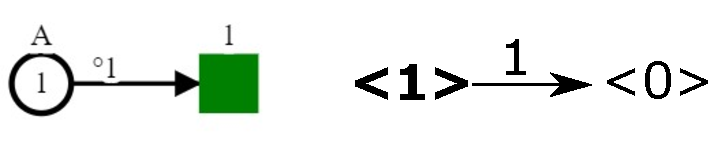
\includegraphics{net_props_01}
    \caption[síť]{}\label{fig:ukázka grafu dosažitelnosti 1}
  \end{subfigure}
  
  \begin{subfigure}[h]{\linewidth}
    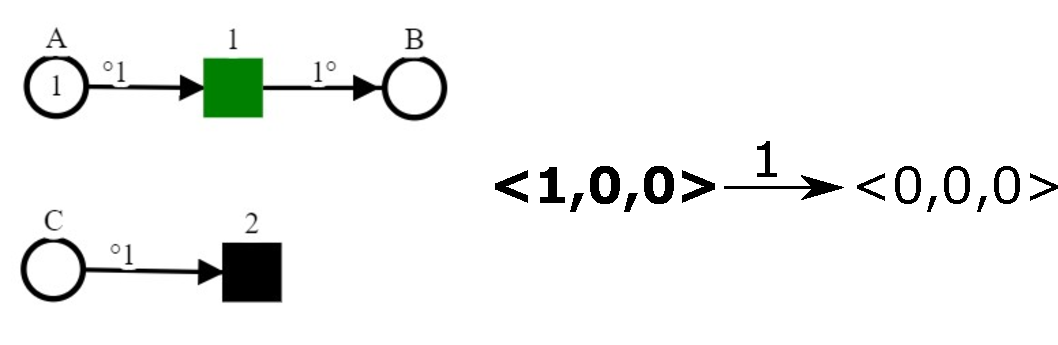
\includegraphics[width=\linewidth]{net_props_02}
    \caption[síť]{}\label{fig:ukázka grafu dosažitelnosti 2}
  \end{subfigure}
  
  \begin{subfigure}[h]{\linewidth}
    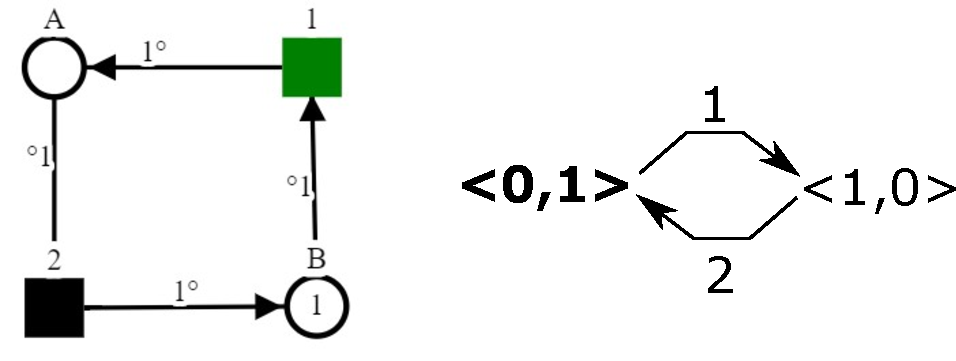
\includegraphics[width=\linewidth]{net_props_03}
    \caption[síť]{}\label{fig:ukázka grafu dosažitelnosti 3}
  \end{subfigure}
  \caption{Ukázky jednoduchých sítí s grafem dosažitelnosti}\label{fig: ukázky jednoduchých sítí}
\end{figure}

Síť na obrázku \ref{fig:ukázka grafu dosažitelnosti 1} \textbf{skončí} a je \textbf{slabě živá}.

Síť na obrázku \ref{fig:ukázka grafu dosažitelnosti 2} \textbf{skončí} a není \textbf{slabě živá}.

A síť na obrázku \ref{fig:ukázka grafu dosažitelnosti 3} je \textbf{vratná} a \textbf{živá}.

Všechny tři sítě jsou ohraničené 1. Také si můžeme všimnout že 
z výše uvedených vlastností u ukázkových sítí 
stačí jen vypsané vlastnosti a ostatní se dají odvodit ze závislosti vlastností.

\clearpage

\subsection{Graf pokrytí}

Hlavní nevýhodou grafu dosažitelnosti je že může být
nekonečný a tudíž je nemožné ho zkonstruovat celý.
Můžeme velice jednoduše navrhnout a sestrojit triviální Petriho síť (Obrázek \ref{fig:neohraničená síť}) u které by konstrukce jejího grafu dosažitelnosti nikdy neskončila.

\begin{figure}[h]
  \centering
  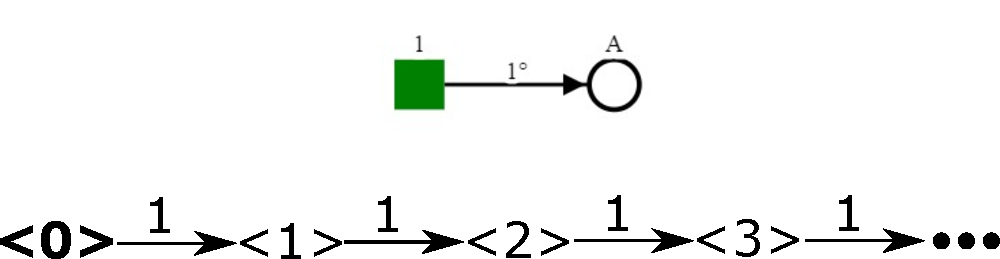
\includegraphics[width=\linewidth]{net_unbounded_reachability}
  \caption{Příklad neohraničené sítě}\label{fig:neohraničená síť}
\end{figure}

Proto existuje upravená verze grafu dosažitelnosti nazvaná grafu pokrytí,
která může obsahovat tzv. $\omega$ ohodnocení které mimo celých 
čísel přiřadí alespoň jednomu místu i hodnotu $\omega$ 
symbolizující že místo může nabívat nekonečně vysokého počtu značek.
Petriho síť se nemůže nacházet v $\omega$ ohodnocení, toto ohodnocení je pouze
pro vytvoření abstrakce v grafu pokrytí.

Protože hodnotu $\omega$ bereme jako nekonečno pak od ní můžeme 
odečíst nebo přičíst libovolně velké číslo a hodnota se nezmění.
$$\dotsb = \omega - 2 = \omega - 1 = \omega = \omega + 1 = \omega + 2 = \dotsb$$

Ohodnocení $M$ značíme jako že je ostře menší $<$ než ohodnocení $M'$
pokud pro každé místo $p$ platí $M(p) \leq M'(p)$ a alespoň pro jedno
místo $p$ platí $M(p) < M'(p)$.
$$
 M<M' = ((\forall p \in P) M(p) \leq M'(p)) \land (\exists p \in P) M(p) < M'(p)
$$

\subsubsection{Sestrojení grafu}

Sestrojování grafu probíhá postupně přidáváním hran. Nejdříve se přidá počáteční 
ohodnocení jako kořen grafu. Následně se z grafu vybírají náhodně
nevypočítané povolené přechody a pokud vedou do místa které ještě 
v grafu není tak se přidá a pokud je ostře menší než ohodnocení ze kterého
je dosažitelné tak se přidají $\omega$ hodnoty na místa ve kterých má více značek.
Algoritmus končí výpočet až jsou všechny povolené 
přechody pro všechny vrcholy v grafu vypočítané.

\begin{center}
  Sestrojení grafu pokrytí pseudokód MakeCoverabilityGraph\ref{alg:MakeCoverabilityGraph}
\end{center}

\begin{algorithm}
  \caption{MakeCoverabilityGraph}\label{alg:MakeCoverabilityGraph}
  \begin{algorithmic}[1]
    \Function{MakeCoverabilityGraph}{$\langle P,T,A,M_0\rangle$}
    \State $\langle V,E,v_0\rangle := \langle\{M_0\},\emptyset,M_0\rangle$
    \State $WorkSet := \emptyset $
    \ForAll{$t \in EnabledTransitions(P,T,A,M_0)$}
    \State $WorkSet := WorkSet \cup \{\langle M_0, t \rangle\} $
    \EndFor

    \While{$WorkSet \neq \emptyset$}
    \State $\langle M, t \rangle := RandomElement(WorkSet)$
    \State $WorkSet := WorkSet \setminus \{\langle M, t \rangle\}$
    \State $M' := FireTransition(P,t,A,M)$
    \ForAll{$\{M'' \;|\; M'' \in V \land (M'' \to^* M \lor M'' = M) \land M'' < M'\}$}
    \ForAll{$p \in P$}
    \State $mp := M(p)$
    \If{$M''(p)<M'(p)$}
    \State $M'(p) := \omega$
    \EndIf
    \EndFor
    \EndFor

    \If{$M' \notin V$}
    \State $V := V \cup \{M'\}$
    \ForAll{$t \in EnabledTransitions(P,T,A,M')$}
    \State $WorkSet := WorkSet \cup \{\langle M', t \rangle\} $
    \EndFor
    \EndIf
    \State $E := E \cup \{\langle M,t,M'\rangle\}$
    \EndWhile

    \State \textbf{return} $\langle V,E,v_0\rangle$
    \EndFunction
  \end{algorithmic}
\end{algorithm}

Pokud sestrojený graf pokrytí neobsahuje žádné $\omega$ ohodnocení,
pak je graf totožný s grafem dosažitelnosti. 
Pokud graf pokrytí obsahuje $\omega$ ohodnocení, zanamená to že 
graf dosažitelnosti by byl nekonečný a tudíž by nebylo možné 
ho zkonstruovat celý a nešli by na něm zjišťovat některé nebo všechy vlastnosti.
Proto si vystačíme s algoritmem na vytváření grafu pokrytí.

\subsubsection{Různé výsledky grafu pokrytí}

Při konstrukci grafu pokrytí záleží v jakém pořadí se hrany přidávají
a výsledný graf může mít různý počet vrcholů a hran 
v závislosti na pořadí přidávání hran.
V našem algoritmu využíváme funkce $RandomElement$ která vybere 
náhodný prvek množiny a snažíme se tak tipovat jaké pořadí hran bude
ideální pro sestrojení nejmenšího grafu. 
Pokud bychom chtěli sestrojit minimální 
graf pokrytí, museli bychom nahradit funkci $RandomElement$ nějakou
funkcí která by vždy vybrala přechody právě 
v takovém pořadí aby došlo k sestrojení minimálního grafu.

Že záleží na pořadí v jakém se hrany přidávájí si můžeme ukázat na 
síti v obrázku \ref{fig:síť různé coverability}. Zde ale musíme 
dávat pozor, protože v tomto případě čísla neznačí přechody,
ale pořadí ve kterém byly hrany přidány.

\begin{figure}[h]
  \centering
  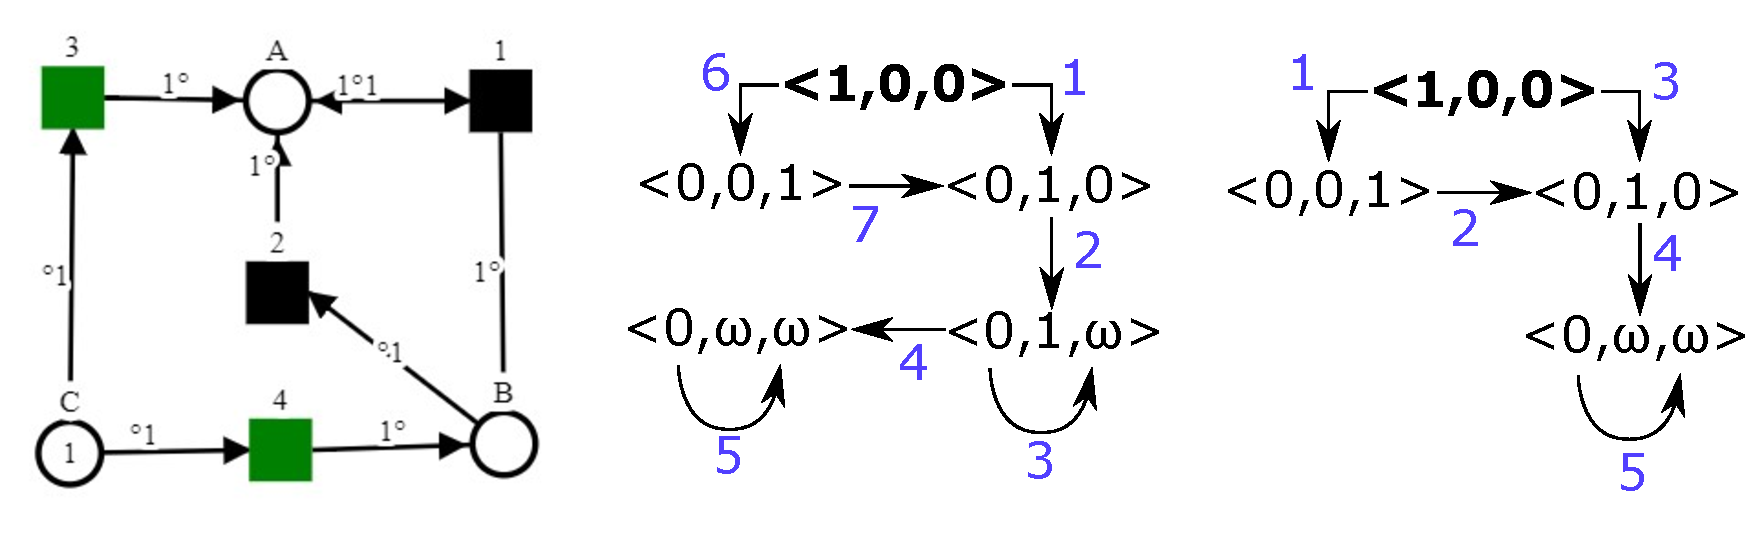
\includegraphics[width=\linewidth]{net_coverability_difference}
  \caption{Příklad sítě z knihy Understanding petri nets\cite{reisig2013understanding}(fig.  14.1) }\label{fig:síť různé coverability}
\end{figure}


\subsubsection{Upravená verze vlastností}

Oproti grafu dosažitelnosti náš graf pokrytí tak jak jsme ho sestrojili 
pomocí algoritmu MakeCoverabilityGraph\ref{alg:MakeCoverabilityGraph} 
nemusí obsahovat všechny výsledky přechodů které mohou nastat a to znamená 
že v některých případech některé vlastnosti Petriho sítě nejsme schopni určit, 
protože nám chybí informace o těchto chybějícíh hranách grafu pokrytí.
Problém je částečně způsobený tím jak máme definovanou hodnotu $\omega$ a pokud 
nějaké místo $p$ je ohodnoceno $\omega$ pak už není možné aby z vrcholu s tímto 
ohodnocením vedla hrana do vrcholu kde místo $p$ nebude mít hodnotu $\omega$.

\begin{figure}[h]
  \centering
  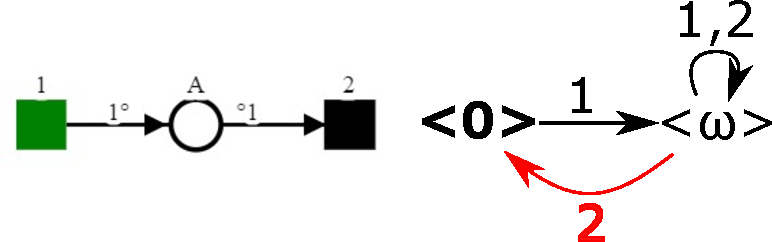
\includegraphics[width=\linewidth]{net_undecidable_reversion}
  \caption{Příklad neohraničené sítě s chybějící hranou v grafu pokrytí}\label{fig:neohraničená síť reversible}
\end{figure}

V Obrázku \ref{fig:neohraničená síť reversible} vidíme červěně zvíražněnou 
hrana která při použití algoritmu MakeCoverabilityGraph\ref{alg:MakeCoverabilityGraph}
chybí. Přitom by tam měla hrana být, protože když budeme neustále opakovat 
aktivaci přechodu 2 tak se eventuálně (až bude počet aktivací přechodu 2 roven počtu aktivací 1) 
dostaneme do ohodnocení kde má místo $A$
hodnotu 0 což je zároveň výchozí ohodnocení. Díky této chybějící hraně 
bychom síť určili jako že není \textbf{vratná} ale přitom ve skutečnosti je.
Proto musíme zjistit jestli jsou všechny vlastnosti grafu dosažitelnosti 
aplikovatlné i na graf pokrytí, případně poupravit nebo rozšířit jejich definici.

Síť je \textbf{ohraničená} pokud graf pokrytí neobsahuje žádné $\omega$ ohodnocení
\begin{proof}
  \textbf{Ohraničenost} sítě je určená konečností grafu dosažitelnosti.
  Nekonečný rozvoj grafu dosažitelnosti je vždy v grafu pokrytí symbolizován
  $\omega$ ohodnocenímy. Z toho můžeme vyvodit že síť je 
  \textbf{ohraničená} pokud její graf pokrytí neobsahuje žádně $\omega$ ohodnocení.
\end{proof}


Petriho síť ne\textbf{skončí} pokud graf obsahuje $\omega$ ohodnocení.
\begin{proof}
  Petriho síť ne\textbf{skončí} pokud je její graf dosažitelnosti nekonečný tudíš
  stejnou úvahou jako u ohraničenosti můžeme říct že síť ne\textbf{skončí}
  pokud její graf pokrytí obsahuje $\omega$ ohodnocení a skončí pokud je splněná
  původní podmínka v definici \ref{def:skončí}.
\end{proof}

Jestli je síť vratná z grafu s $\omega$ ohodnocením jsme si už ukázali 
že díky chybějícím hranám určitelné není. Můžeme si ale jednoduchou 
úvahou určit množinu případů kdy síť rozhodně vratná není, a to v 
situaci kdy existuje $\omega$ ohodnocení a neexistuje žádný přechod 
který by měl větší vstup jak výstup.
\begin{proof}
  Pokud máme $\omega$ ohodnocení tak to mimo jiné znamená že se suma značek všech 
  míst může při opakovaném aktivování
  některých přechodů zvyšovat neustále. Pak musí existovat i přechod
  terý tuto sumu snižuje, neboli přecho který má vyšší sumu
  násobků z místa $^\to t$ než do místa $t ^\to$. Pokud takový 
  přechod neexistuje přesto že v coverability grafu je $\omega$ ohodnocení,
  pak můžeme s jistotou říct že síť není \textbf{vratná}
\end{proof}
Pro určení jestli je síť \textbf{vratná} v ostatních případech
bychom potřebovali algoritmus který vytváří i zpětné hrany z $\omega$ ohodnocení.


Petriho síť je \textbf{bez mrtvého bodu} pokud z každého vrcholu grafu 
pokrytí vede alespoň jedna hrana.
\begin{proof}
  V tomto případě nemusíme rozlišovat $\omega$ ohodnocení a standardní ohodnocení,
  pokud z něj vede v grafu hrana, znamená to že v tomto ohodnocení síť neuvázne.
\end{proof}

Petriho síť je \textbf{slabě živá} pokud pro každý přechod existuje 
v grafu hrana označená tímto přechodem.
\begin{proof}
  $\omega$ ohodnocení stejně jako v případě 
  určování jestli je síť \textbf{bez mrtvého bodu} 
  výsledek neovlivní.
\end{proof}

Petriho síť je \textbf{živá}\index{síť živá} pokud 
pro každý přechod $t$ a každé ohodnocení $M$ existuje v grafu cesta
z ohodnocení $M$ do ohodnocení ze kterého vede hrana z označením přechodu $t$.
\begin{proof}
 Když jsou ohodnocení $M < M'$, pak pokud je přechod $t$ 
  povolený v $M$ pak musí být povolený i v $M'$. Díky tomu můžemě určit
  že chybějící hrany z ostře větších ohodnocení do menších nejsou potřeba protože 
  by jejich existence stejně neumožňovala přístup k dalším přechodům a proto můžeme 
  živost vyčíst i grafu pokrytí.
\end{proof}

\subsection{Příklady sítí}
\todo{síť + analýza v programu}




\clearpage
\section{Editor}
\subsection{Systémové požadavky}
\begin{itemize}
  \item Operační systém: Windows 10 (starší verze windows netestovány)
  \item Ovládání: klávesnice+myš
\end{itemize}

  
\subsection{Rozložení editoru}
Editor je rozložený na několik částí. Všechny tyto části 
jsou písmeny označené v Obrázku \ref{fig:Rozložení editoru} 
Rozložení editoru.Každá část editoru je popsaná ve své vlastní sekci.

\begin{figure}[h]
  \centering
  \begin{subfigure}[h]{350px}
    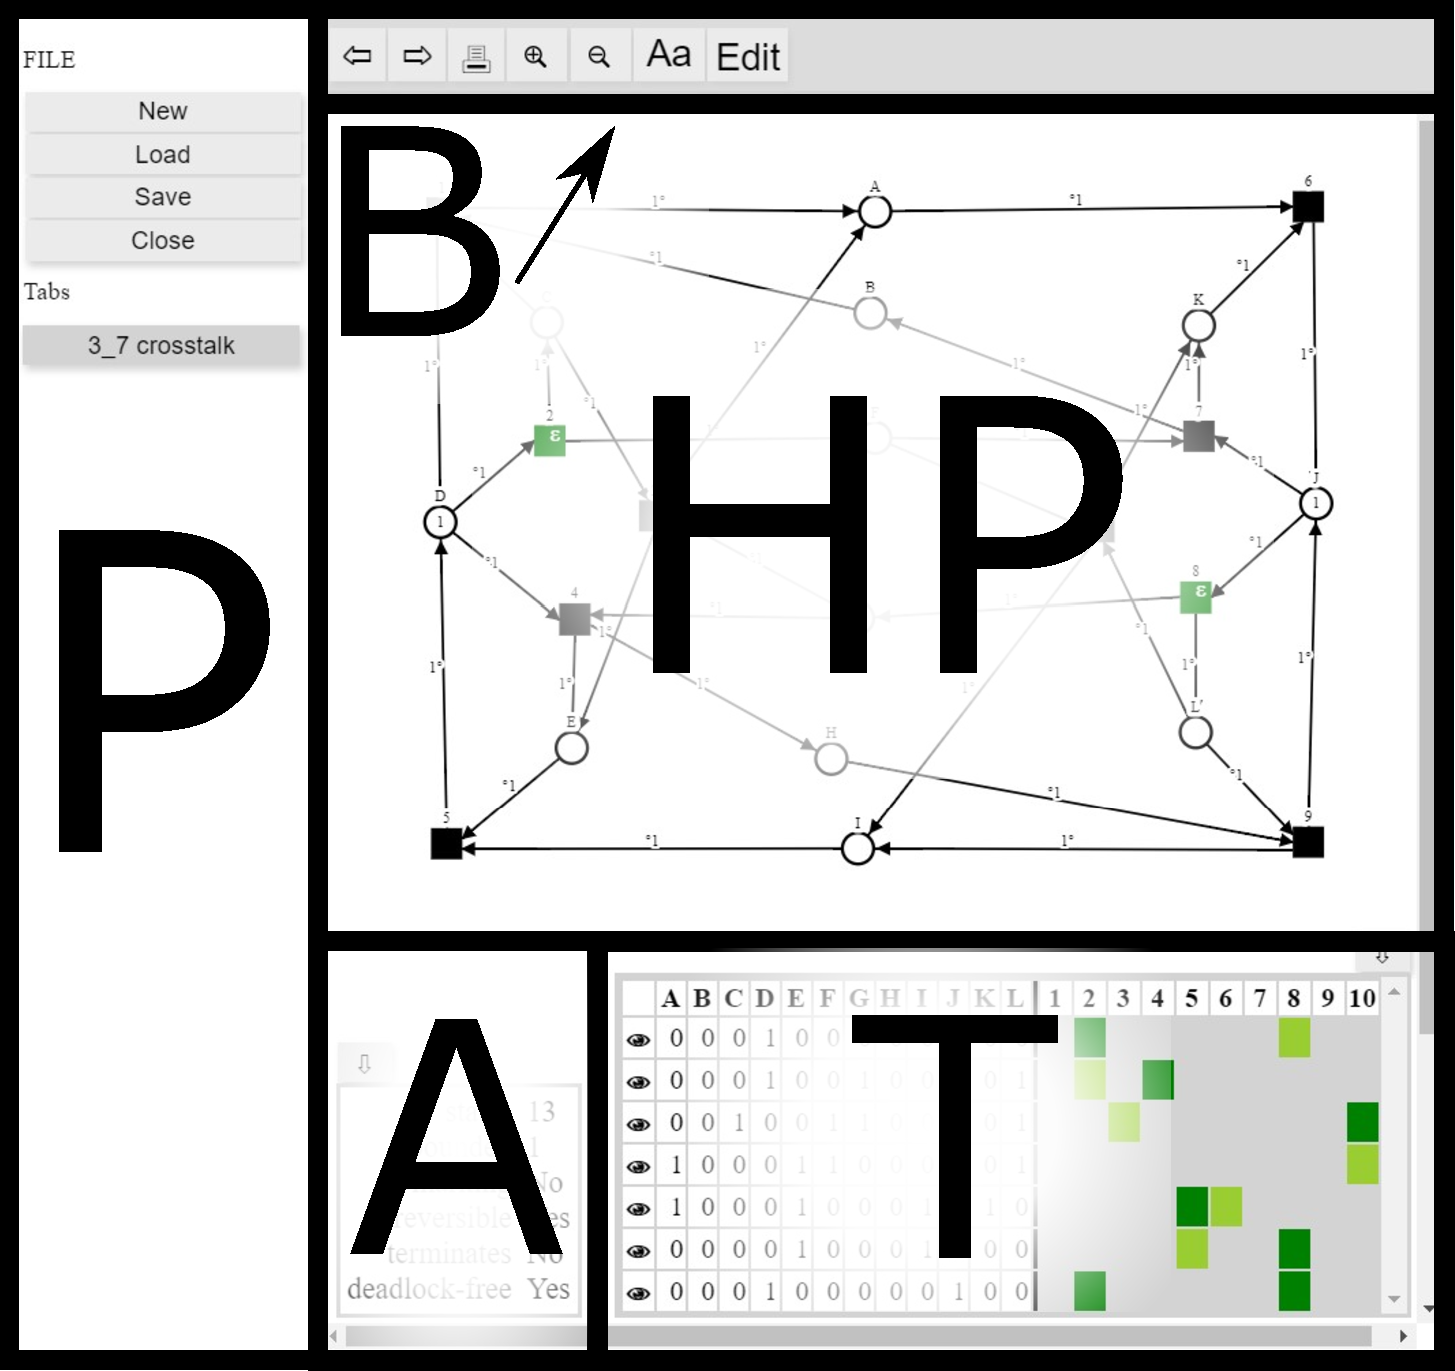
\includegraphics[height=300px, width=350px]{full_image_splited}
  \end{subfigure}
  \caption{Rozložení editoru}
  \label{fig:Rozložení editoru}
  \begin{subfigure}[h]{0.55\textwidth}
    \begin{tabular}{|c l c|}
      \hline
      označení &      název části editoru &    sekce \\
      \hline
      \hline
      P &             Postranní panel&  \ref{panel} \\
      HP &            Hlavní plocha editoru&  \ref{hlavní plocha} \\
      B &             Panel nástrojů editoru &  \ref{panel nástrojů} \\
      T &             Tabulka ohodnocení &  \ref{tabulka ohodnocení} \\
      A &             Výsledky analýzy &  \ref{výsledky analýzy} \\
      \hline
    \end{tabular}
  \end{subfigure}
\end{figure}


\subsubsection{Postranní panel}\label{panel}

Postraní panel obsahuje tlačítka pro práci se záložkami a 
samotné záložky. Pod označením \textbf{FILE} jsou tlačítka:
\begin{center}
  \begin{tabular}{c p{0.8\linewidth}}
    \textbf{New}    & Vytvoří novou prázdnou záložku \\
    \textbf{Load}   & Otevře dialog pro načtení uložené sítě \\
    \textbf{Save}   & Uloží síť v otevřené záložce. Pokud byla síť již uložena 
      nebo načtena dialog nabídne uživateli na výběr dvě možnosti.
      Možnost \textit{yes} uloží a přepíše původní soubor.
      Možnost \textit{Select file} otevře dialog 
      a uživatel vybere vlastní místo uložoní. \\
    \textbf{Close}  & Zavře aktuálně otevřenou záložku \\
  \end{tabular}
\end{center}

Pod označením \textbf{Tabs} jsou pak záložky které se otevírají kliknutím.
Záložky jsou nazvané podle jména souboru sítě.

\begin{figure}[h]
  \centering
  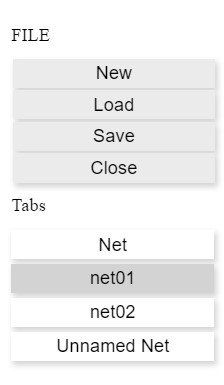
\includegraphics{editor_panel}
  \caption{\\Postranní panel}\label{fig:Postranní panel}
\end{figure}

\subsubsection{Ovládání, Hlavní plocha editoru}\label{hlavní plocha}

Editor je navržený tak aby bylo možné jej používat pouze za použítí 
myši bez potřeby využívání klávesnice. Zároveň oproti ostatním editorům
nemá různé nástroje (např. na vkládání různých objektů) a všechny 
akce editování jsou možné bez toho aby kurzor opustil hlavní plochu editoru.

Kliknutím levým tlačítkem myši se vytvoří přechod. 
Kliknutím na přechod se začne vytvářet hrana. Pokud se při 
vytváření hrany klikne do nějakého místa tak se na něj hrana 
připojí. Pokud se klikne do prázdného prostoru vytvoří se zde nové místo.
vytváření hrany jde zrušit pravým tlačítkem myši.

Při kliknutí na hranu nebo místo se otevře dialog na obrázku \ref{fig:editace hodnot} editace hodnoty.
Při najetí nad editované pole se zobrazí šipky kterými 
je možné přidávat nebo ubírat hodnotu, nebo je možné taky 
do něj kliknout aby se do zde umístil kurzor klávesnice a 
přitom když je myš stále nad polem použít kolečko na změnu hodnoty.
Dialogy se ukládají kliknutím na OK, kliknutí do jiného místa(levé i pravé) 
hlavní plochy způsobí zavření dialogu bez provedení změny.

Ohodnocení místa se dá měnit i bez otevření dialogu a to najetím myši
a rolováním kolečka, zatímco při najetí a rolovaní na hranu pouze prohodí směr
hrany. Rolovaní při najetí na přechody pouze odebere nebo přidá přechodu 
$\epsilon$ označení(označení pouze orientační pro uživatele).

Kliknutím a tažením je pak možné jednotlivá místa a přechody přesouvat.
Při přesouvání se jednotlivé objekty navzájem odpuzují aby nedošlo k jejich překrytí.

\begin{figure}[h]
  \centering
  \begin{subfigure}[h]{0,4\linewidth}
    
\includegraphics{dialog_place}
    \caption{editace ohodnocení místa}
  \end{subfigure}
  \begin{subfigure}[h]{0,4\linewidth}
    
\includegraphics{dialog_arc}
    \caption{editace hodnot hrany}
  \end{subfigure}
  \caption{Editace hodnot}
  \label{fig:editace hodnot}
\end{figure}


\todo{módy + odkaz na tlačítko}

\subsubsection{Panel nástrojů editoru}\label{panel nástrojů}

Funkce tlačítek panelu nástrojů zobrezeného v obrázku \ref{fig:Panel nástrojů editoru}:
\begin{center}
  \begin{tabular}{r p{0.8\linewidth}}
    \textbf{Zpět/Vpřed}          & Vrátí poslední akci nebo zruší vrácení poslední akce \\
    \textbf{Tisk}                & Otevře dialog pro tisk otevřené sítě \\
    \textbf{Přiblížit/Oddálit}   & Přiblíží/Oddálí Petriho síť \\
    \textbf{Skrýt/Zobrazit popisky}  & Skryje nebo zobrazí popisky míst a přechodů \\
    \textbf{Změna módu}  & Přepíná mezi \textbf{editovacím módem} a módem \textbf{spouštění sítě}. \\
  \end{tabular}
\end{center}


\begin{figure}[h]
  \centering
  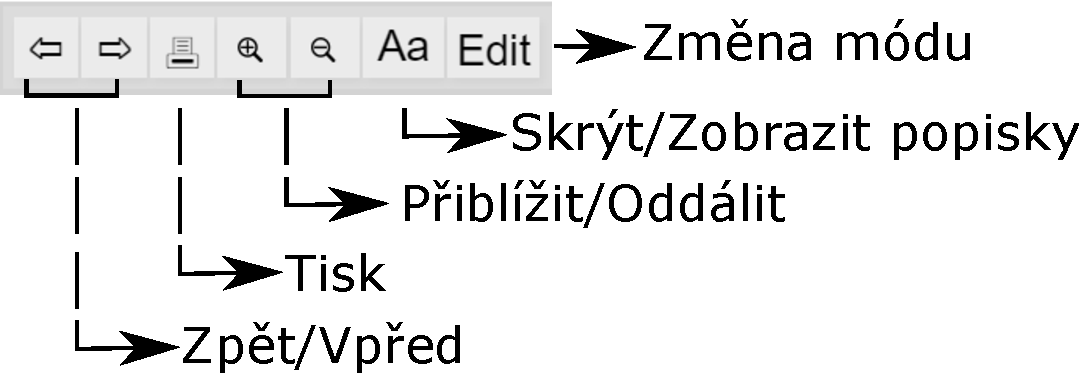
\includegraphics[width=\linewidth]{bar}
  \caption{Panel nástrojů editoru}\label{fig:Panel nástrojů editoru}
\end{figure}

\subsubsubsection{Tisk}

Pro uložení sítě na disk je potřeba ještě vir


\subsubsection{Tabulka ohodnocení}\label{tabulka ohodnocení}

Tabulka ohodnocení (Obrázek \ref{fig:Tabulka ohodnocení obrázek}) slouží pro rychlé testování sítě uživatelem.
Každý řádek v tabulce reprezentuje jedno dosažitelné ohodnocení 
v levé části tabulky a povolené přechody v tomto ohodnocení jsou 
zobrazeny zelenými obdelníčky v pravé části tabulky.
Uživatel může kdykoliv kliknout na jakýkoliv ze zelených obdelníčků 
a tím přidá další řádek pod řádek na který kliknul který obsahuje 
nové ohodnocení vzíklé aplikací přechodu který uživatel vybral.
Pokud uživatel vybral přechod na řádku pod kterým už řádky jsou, 
tak budou všechny odebrány a pak až se přidá nový.

Pokud uživatel najede na ikonu oka tak dojde k zobrazení ohodnocení 
daného řádku do sítě na hlavní ploše editoru.

\begin{figure}[h]
  \centering
  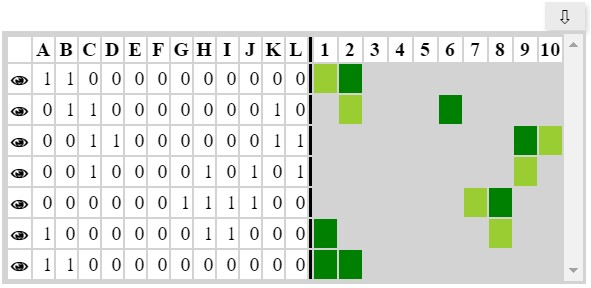
\includegraphics[width=\linewidth]{tabulka}
  \caption{Tabulka ohodnocení}\label{fig:Tabulka ohodnocení obrázek}
\end{figure}


\subsubsection{Výsledky analýzy}\label{výsledky analýzy}


\subsubsection{Klávesové zkratky}





\section{Použité technologie}

\subsection{nodejs}
Aplikace je psaná za pomoci opensourcové technologie nodeJS, která umožňuje využívat jazyk
JavaScript pro psaní serverových aplikací. Cílem platformy nodeJS je vytvořit
ekosystém pro jednoduší vývoj webových stránek a aplikací kde stačí pro vyrvaření
funkcionality pouze jeden programovací jazyk.

\subsection{Typescript}
Typescript je opensource programovací jazyk od společnosti Microsoft který je nadstavbou nad jazykem JavaScript.
Jelikož je Typescript nadstavbou nad programovacím jazykem JavaScript tak je jakýkoliv validní kód v JavaScriptu automaticky validním kódem v Typescriptu.
Typecript se kompiluje do Javascriptu a proto po stránce funkcionality nenabízí nic navíc avšak po stránce vývoje nabízí možnost statické typové kontroly
se kterou je spjaté fungování našeptávačů v dnešních textových editorech a také nabízí možnost kompilace do starších verzí JavaScript se simulací funkcionality novejších verzí JavaScriptu.
\todo{příklady kódu ?}


\subsection{Electron}
Electron je opensource framework pro vytváření desktopových aplikací pomocí webových technologií JavaScript, HTML a CSS.
Využívá NodeJS


\subsection{Javascriptová Knihovna Data driven documents (D3)}
\todo{příklady kódu ?}

\subsection{Scalable Vector Graphics (SVG)}
\todo{příklady kódu ?}




\section{Stavba programu}

\subsection{Třída 1}
\subsection{Třída 2}
\subsection{Třída 3}
\subsection{Třída 4}























































































\section{Obsah přiloženého CD/DVD} \label{sec:ObsahCD}

Na samotném konci textu práce je uveden stručný popis obsahu
přiloženého CD/DVD, tj.~jeho závazné adresářové struktury, důležitých
souborů apod.

\begin{description}

  \item[\texttt{bin/}] \hfill \\
        Instalátor \textsc{Instalator} programu, popř.~program
        \textsc{Program}, spustitelné přímo z~CD/DVD. / Kompletní adresářová
        struktura webové aplikace \textsc{Webovka} (v~ZIP archivu) pro
        zkopírování na webový server. Adresář obsahuje i~všechny runtime
        knihovny a~další soubory potřebné pro bezproblémový běh instalátoru
        a~programu z~CD/DVD / pro bezproblémový provoz webové aplikace na
        webovém serveru.

  \item[\texttt{doc/}] \hfill \\
        Text práce ve formátu PDF, vytvořený s~použitím závazného stylu KI
        PřF UP v~Olomouci pro závěrečné práce, včetně všech příloh,
        a~všechny soubory potřebné pro bezproblémové vygenerování PDF
        dokumentu textu (v~ZIP archivu), tj.~zdrojový text textu, vložené
        obrázky, apod.

  \item[\texttt{src/}] \hfill \\
        Kompletní zdrojové texty programu \textsc{Program} / webové aplikace
        \textsc{Webovka} se všemi potřebnými (příp.~převzatými) zdrojovými
        texty, knihovnami a~dalšími soubory potřebnými pro bezproblémové
        vytvoření spustitelných verzí programu / adresářové struktury pro
        zkopírování na webový server.

  \item[\texttt{readme.txt}] \hfill \\
        Instrukce pro instalaci a~spuštění programu \textsc{Program}, včetně
        všech požadavků pro jeho bezproblémový provoz. / Instrukce pro
        nasazení webové aplikace \textsc{Webovka} na webový server, včetně
        všech požadavků pro její bezproblémový provoz, a~webová adresa, na
        které je aplikace nasazena pro účel testování při tvorbě posudků
        práce a~pro účel obhajoby práce.

\end{description}

Navíc CD/DVD obsahuje:

\begin{description}

  \item[\texttt{data/}] \hfill \\
        Ukázková a~testovací data použitá v~práci a~pro potřeby testování
        práce při tvorbě posudků a~obhajoby práce.

  \item[\texttt{install/}] \hfill \\
        Instalátory aplikací, runtime knihoven a~jiných souborů potřebných
        pro provoz programu \textsc{Program} / webové aplikace
        \textsc{Webovka}, které nejsou standardní součástí operačního
        systému určeného pro běh programu / provoz webové aplikace.

  \item[\texttt{literature/}] \hfill \\
        Vybrané položky bibliografie, příp.~jiná užitečná literatura
        vztahující se k~práci.

\end{description}

U~veškerých cizích převzatých materiálů obsažených na CD/DVD jejich
zahrnutí dovolují podmínky pro jejich šíření nebo přiložený souhlas
držitele copyrightu. Pro všechny použité (a~citované) materiály,
u~kterých toto není splněno a~nejsou tak obsaženy na CD/DVD, je uveden
jejich zdroj (např.~webová adresa) v~bibliografii nebo textu práce
nebo v souboru \texttt{readme.txt}.

%% -------------------------------------------------------------------

%% Sazba volitelného seznamu zkratek, za přílohami.
\printglossary

%% Sazba povinné bibliografie, za přílohami (případně i za seznamem
%% zkratek). Při použití BibLaTeXu použijte makro
%% \printbibliography. jinak prostředí thebibliography. Ne obojí!

%% Sazba i v textu necitovaných zdrojů, při použití
%% BibLaTeXu. Volitelné.
\nocite{*}
%% Vlastní sazba bibliografie při použití BibLaTeXu.
\printbibliography

%% Bibliografie, včetně sazby, při nepoužití BibLaTeXu.
% \begin{thebibliography}{9}
%\bibitem{kniha2} \uppercase{Hawke}, Paul. NanoHttpd: Light-weight HTTP server designed for embedding in other applications. GitHub [online]. 2014-05-12. [cit. 2014-12-06]. Dostupné z: \url{https://github.com/NanoHttpd/nanohttpd}
%
%\bibitem{jeske13} \uppercase{Jeske}, David; \uppercase{Novák}, Josef. Simple HTTP Server in \csharp: Threaded synchronous HTTP Server abstract class, to respond to HTTP requests. CodeProject: For those who code [online]. 2014-05-24. [cit. 2014-12-06]. Dostupné z: \url{http://www.codeproject.com/Articles/137979/Simple-HTTP-Server-in-C}
%
%\bibitem{uzis2012} \uppercase{ÚSTAV ZDRAVOTNICKÝCH INFORMACÍ A STATISTIKY ČR}. Lékaři, zubní lékaři a farmaceuti 2012 [online]. Praha 2, Palackého náměstí 4: Ústav zdravotnických informací a statistiky ČR, 2012 [cit. 2014-12-06]. ISBN 978-80-7472-089-5. Dostupné z: \url{http://www.uzis.cz/publikace/lekari-zubni-lekari-farmaceuti-2012}
% \end{thebibliography}

%% Sazba volitelného rejstříku, za bibliografií.
\printindex

\end{document}
